Relaciona con una linea recta cada enunciado con la expresión algebraica que le corresponde. Considera los datos de la tabla \ref{fig:SINMAT1_U3_AC72_IMG1}.
\begin{figure}[H]
    \centering
    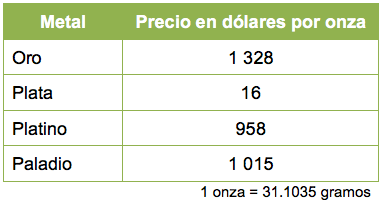
\includegraphics[width=0.5\textwidth]{../images/SINMAT1_U3_AC72_IMG1}
    \caption{Tabla de precios de algunas divisas.}
    \label{fig:SINMAT1_U3_AC72_IMG1}
\end{figure}
\begin{multicols}{2}
    \begin{choices}
        \choice $y = 1 015x$
        \choice $y = 0.0010x$
        \choice $y = 1 328x$
        \choice $y = 0.0625x$
    \end{choices}
    \columnbreak
    \begin{parts}
        \part \fillin[C][1.5cm] Dólares necesarios para comprar cierto número de onzas de oro.	\vspace{1cm}
        \part \fillin[B][1.5cm] Onzas de platino que se pueden comprar con cierta cantidad de dólares.	\vspace{1cm}
        \part \fillin[D][1.5cm] Onzas de plata que se pueden comprar con cierta cantidad de dólares.	\vspace{1cm}
        \part \fillin[A][1.5cm] Dólares necesarios para comprar cierto número de onzas de paladio.
    \end{parts}
\end{multicols}